\documentclass[12pt,fleqn,twocolumn]{article}

\usepackage[english]{babel}
\usepackage[utf8]{inputenc}

\PassOptionsToPackage{hyphens}{url}\usepackage{hyperref}

\usepackage[top=2.5cm, bottom=2.5cm, left=3cm, right=3cm, includeheadfoot]{geometry}

\usepackage{fancyhdr}
\usepackage{graphicx}
\usepackage{float}
\usepackage{changepage}
\usepackage[nottoc, numbib]{tocbibind}
\usepackage{lastpage}
\usepackage{setspace}
\usepackage[bottom]{footmisc}
\usepackage{titling}

\usepackage{amsmath}
\usepackage{amssymb}
\usepackage{nicefrac}
\usepackage{icomma}

\usepackage{csquotes}
\usepackage[backend=biber, style=alphabetic, citestyle=alphabetic, maxcitenames=4, maxbibnames=4, mincitenames=2]{biblatex}

\mathcode`\*=\number\cdot
\newcommand{\numberthis}{\addtocounter{equation}{1}\tag{\theequation}}
\newcommand{\acomm}[1]{\hspace{2.5cm}\text{#1}}
\newcommand{\code}[1]{{\texttt{\small#1}}}

\newcommand{\pro}{\ensuremath{\:\%{}\:}}
\newcommand{\md}{\ensuremath{\text{d}}}
\newcommand{\NN}{\ensuremath{\mathbb N}}
\newcommand{\ZZ}{\ensuremath{\mathbb Z}}
\newcommand{\QQ}{\ensuremath{\mathbb Q}}
\newcommand{\RR}{\ensuremath{\mathbb R}}
\newcommand{\CC}{\ensuremath{\mathbb C}}
\newcommand{\DD}{\ensuremath{\mathbb D}}
\newcommand{\LL}{\ensuremath{\mathbb L}}
\newcommand{\PP}{\ensuremath{\mathbb P}}
\newcommand{\transpose}[1]{\ensuremath{#1^{\textup T}}}

\newcommand{\half}{\ensuremath{\frac{1}{2}}}
\newcommand{\third}{\ensuremath{\frac{1}{3}}}
\newcommand{\fourth}{\ensuremath{\frac{1}{4}}}
\newcommand{\ctp}[1]{\ensuremath{\cdot10^{#1}}}
\newcommand{\reci}{\ensuremath{^{-1}}}

\usepackage[acronym, toc]{glossaries}
\newacronym{dl}{DL}{Deep Learning}
\newacronym{nlp}{NLP}{Natural Language Processing}
\newacronym{dp}{DP}{Differential Privacy}
\newacronym{ml}{ML}{Machine Learning}
\newacronym{dpsgd}{DP-SGD}{Differentially Private Stochastic Gradient Descent}
\newacronym{fl}{FL}{Federated Learning}
\newacronym{dpfa}{DP-FedAvg}{Differentially Private Federated Averaging}
\newacronym{adlm}{AdLM}{Adaptive Laplace Mechanism}

\glsdisablehyper


\addbibresource{references.bib}

\setlength{\droptitle}{-10ex}

\title{Winning Weights: A Review of The Lottery Ticket Hypothesis}

\author{Søren Winkel Holm}
\date{\today}

\pagestyle{fancy}
\fancyhf{}
\lhead{Søren Winkel Holm}
\chead{}
\rhead{Technical University of Denmark}
\lfoot{The Lottery Ticket Hypothesis}
\rfoot{Page \thepage{} of \pageref{LastPage}}

\graphicspath{{imgs/}}
\linespread{1.15}

\begin{document}
\setlength{\headheight}{15pt}
\addtolength{\topmargin}{-2.5pt}

\maketitle
\thispagestyle{fancy}
% \tableofcontents

\section*{Introduction}%
\label{sec:Introduction}
While \acrfull{dl} is celebrated as a universal technological step forward, making complex modelling available to many industries, the computational cost of the training procedure of \acrfull{dnn}'s makes the technology unaccessible for low-resource actors.
The price of large language modelling projects such as Google's T5 is estimated in the region of \$ 10 M \cite{Sharir2020TheCO} and such tech companies have a leading role in research \cite{ivanov2020icml, ivanov2020neurips}.
% https://arxiv.org/pdf/2004.08900.pdf
While the processing of big data is naturally computationally intensive, much of training cost is caused by a large number of epochs being required before convergence.
\acrfull{lth} points to \acrshort{dnn} learning dynamics that are keeping this number high.

\begin{figure}
    \centering
        \includegraphics[page=3, clip, trim=5cm 21.5cm 12.5cm 2.7cm, width=.8\linewidth]{pruning.pdf}
        \includegraphics[page=3, clip, trim=10cm 21.85cm 4cm 2.7cm, width=\linewidth]{pruning.pdf}
        \caption{The original iterative pruning method where connectivity training corresponds to standard full training of a dense \acrshort{dnn} \cite[Fig. 2 and 3]{han2015learning}.}
    \label{fig:pruning.pdf}
\end{figure}\noindent
To help availability, rich actors often share the trained model parametrizations but even in this case, application might be widely inaccessible because of computational costs of inference using these large parametrizations.
This problem has been attacked using model pruning, reducing trained model size while retaining performance, but the expensive training of the full \acrshort{dnn} has generally been required.
\acrshort{lth} explains why an initial full training is generally required and opens up for researching how to train efficient parametrizations from scratch.
These ideas and methods will here be reviewed.

\section*{Fundamental Concepts}%
\acrshort{dnn} pruning refers to disabling particular model connections $w_i \leftarrow 0$ possibly to improve generalization, reducing memory constraints in inference and lowering inference computation \cite{LeCun1989OptimalBD}.
Pruning during training is related to regularization e.g. using dropout, while pruning after fully training a dense network parametrization often is motivated by computational cost, and might require some fine-tuning to limit the decrease in accuracy \cite{lange2020lth}.
Disabling unnecessary weights is a way to learn the connectivity of a \acrshort{dnn} and can be performed iteratively based on magnitude such as 
\begin{equation}\label{eq:crit}
    \forall i \text{ s. t. } |w_i^{(t)}|<k \text{ let } w_i^{(t+1)} \leftarrow 0,
\end{equation}
where each iteration is followed by fine-tuning and $k$ is a threshold set to e.g. $k=s\sqrt{\operatorname{Var}[w]}, s=\half$ \cite{han2015learning, nzmora2019distiller}. 
The procedure is stopped when a specified compression level of performance drop is reached \cite{han2015learning} as shown on Figure \ref{fig:pruning.pdf}.
The pruned parametrizations $w^{(p)}$ can be represented using a mask $m$, $w^{(p)} = m \odot w$ and \eqref{eq:crit} is thus dubbed a masking criterion.
Pruning might be structured locally by assigning layer-specific thresholds and target compression levels or by fixing parts of the \acrshort{dnn} \cite{han2015learning}.
The resulting sparse \acrshort{dnn} $f(x;m\odot w)$ is called a subnetwork of the full, trained $f(x;w)$

Simple pruning approaches have empirically been shown to work well across network types and learning tasks with compression rates of $\sim \times 10$ resulting in accuracy drops of $\sim 1\pro$ \cite[Fig. 7] {bla2020state}.
These results do not arise when training from the start with randomly pruned networks \cite[Chap. 4]{li2016filt}, \cite[Chap. 3.3]{han2015learning}.
\acrshort{lth} gives an explanation for this effect by postulating the existence of a \emph{winning ticket} for a randomly initialized, dense \acrshort{dnn} $f(x;w^{(0)}), w^{(0)}\sim \mathcal D_w$.
A winning ticket is a subnetwork $f(x;m\odot w^{(0)})$ that can be trained by itself and reach same generalization error as the full network in the same number of epochs or less.
The name thus implies the existence of an initialization lottery where specific combinations of connection masks and weight prior realisations allow learning.
In this context, standard pruning techniques find winning tickets by first learning the entire, dense $w$ and then after training finding $m$.

\acrshort{lth} implies that $m$ can be computed from a full training after which the weights can be \emph{rewinded} to $w^{(0)}$ at which point the training $m \odot w^{(0)}$ should result in a performant network.

\section*{State of the Art}%
\subsubsection*{Evidence for ticket existence}
\acrshort{lth} was presented by \textcite{frankle2018the} in \citeyear{frankle2018the} where empirical evidence for the hypothesis was presented on MNIST and CIFAR-10.
An effect was seen when comparing training of rewinded weights of a winning ticket to random reinitialization.
Using iterative pruning, winning tickets were found for all tried \acrshort{dnn}'s and these were found to learn faster than full networks, but for deep networks such as VGG-19, finding the tickets was sensitive to learning rate setup and required warmup steps \cite[Chap. 4]{frankle2018the}.

In follow-up work, the robustness of this iterative search for winning tickets was improved by introducing a procedure called \emph{instability analysis} where the impact of \acrfull{sgd} noise such as minibatch order and augmentations was investigated \cite{Frankle2020LinearMC}.
This analysis showed that for many deeper networks, stability against \acrshort{sgd} noise occurs after a number of training steps $k$.
For \acrshort{lth} to hold robustly on these \acrshort{dnn}'s, rewinding of weights was changed from $m \odot w^{(0)}$ being the winning ticket to $m\odot w^{(k)}$ being winning.
Thus, the winning ticket was not shown to exist at initialization but slightly-trained winning subnetworks were empirically found across challenging datasets and network sizes.
These winners were dubbed winning matching tickets instead of winning lottery tickets and this weaker hypothesis has been called \acrfull{lthr} \cite{lange2020lth} .

Concurrently, analysis quantifying the performance of winning tickets compared to previous pruning methods was performed by \textcite{Renda2020ComparingRA}.
The rewinding to winning matching tickets and retraining of \acrshort{lthr} ended up outperforming standard pruning that fine-tunes final weights.
Furthermore, the rewinding approach was superior in a limited-budget setting across \acrfull{nlp} and \acrfull{cv} tasks, and it was concluded that \acrshort{lthr} was \acrfull{sota} for pruning in terms of accuracy, compression and computational cost \cite[Chap. 6]{Renda2020ComparingRA} \cite{lange2020lth}.

In \citeyear{Malach2020ProvingTL}, \acrshort{lth} was theoretically proven for fully-connected ReLU \acrshort{dnn}'s by \textcite{Malach2020ProvingTL} using the theory of random networks.
In the same paper, an even stronger conjecture was proven:
For every \acrshort{dnn} of sufficient size, there exists an subnetwork achieving matching performance in itself without additional training \cite[Theorem 2.1]{Malach2020ProvingTL}.

\subsubsection*{Early ticket identification}
The simple train-rewind-retrain approach used to empirically demonstrate the existance of winning matching tickets was revealed to give strong pruning performance across tasks without need for hyperperameter tuning \cite[Chap. 6]{Renda2020ComparingRA}.
However, this method requires full convergence of the network before identifying the optimal ticket.
Training of sparse \acrshort{dnn}'s would improve dramatically if the winning ticket mask $m$ could be found before training.

In \citeyear{You2020DrawingET}, identification of winning tickets was performed early in training by \textcite{You2020DrawingET}.
These \acrfull{eb} tickets were found using a mask distance measure between epochs.
A mask $m_t$ was at each epoch computed and the Hamming distance between the binary matrices $m_{t-1}$ and $m_{t}$ was used as a ticket search criterion \cite[Chap. 3.3]{You2020DrawingET}.
Search was stopped when the criterion was under $\epsilon = 0.1$ for five consecutive epochs, resulting in an algorithm that succesfully found winning tickets at much less computational cost.
Across \acrshort{cv} tasks, \acrshort{eb} tickets performed at the same accuracy level compared to standard winning tickets and other pruning techniques while using less than half the number of computations.

Also in 2020, two approaches attempted to fully exploit \acrshort{lth} by finding $m$ at initialization were presented.
One by \textcite{Wang2020PickingWT} called \acrfull{grasp} which required computation of a Hessian-gradient product $\mathbf H \mathbf g$ using a batch of training data after which $m$ is constructed by tresholding network scores $w \odot \mathbf H \mathbf g$.
The score computation was theoretically motivated through linearised training dynamics \cite[Chap. 4.1]{Wang2020PickingWT} which have been described for wide \acrshort{dnn}'s using a kernel over training data \cite{Lee2019WideNN}.
Another approach also analysed gradient flow at initialization, but this method named \acrfull{synflow} produced by \textcite{Tanaka2020PruningNN}, did not use any training data.
The researchers identified a key problem with aggressive pruning that especially must be addressed when designing a priori pruning mechanisms: \emph{layer-collapse}, wherein an entire layer is pruned.
Using avoidance of this problem as a guiding principle, the researchers introduced \emph{synaptic saliency}, a score metric which provenly did not induce layer-collapse.
The ticket was then constructed by optimising the weights against a synaptic saliency loss function based on layer-wise products of absolute weight values \cite[Chap. 6]{Tanaka2020PruningNN}.

Both methods were tested on \acrshort{cv} tasks and achieved comparative performance to standard \acrshort{lth} with \acrshort{synflow} outperforming all other methods at extreme compression ratios where \acrshort{grasp} and standard magnitude-based \acrshort{lth} suffer from layer-collapse \cite[Chap. 7]{Tanaka2020PruningNN}.
For multiple architectures, especially of the ResNet type, \acrshort{grasp} is, however, slightly \acrshort{sota} at more reasonable compression ratios of $\times 100$ to $\times 10$\cite[Tab. 4]{Wang2020PickingWT}\cite[Fig. 6]{Tanaka2020PruningNN}.
Also, the influential pruning algorithm \acrfull{snip} contains ideas used in both these methods and performs similarly to \acrshort{grasp} also using training data, but is not formulated in the \acrshort{lth} context \cite{Lee2019SNIPSN}.

\section*{Open Problems}%
\label{sec:Open Problems}
\begin{itemize}
    % \item \emph{What are we talking about when finding winning tickets?}
    %     Though the foundational 
    \item \emph{Do tickets generalize?}
        In the original form, a winning ticket is winning for a specific initialization for a specific learning problem and optimization procedure.
        If, for this specific task, the ticket gradient flow is optimal, it might be natural to assume that the ticket is also relevant for other, similar problems.
        Current applications of such ideas show promising results, but are limited to \acrshort{cv} and require care for optimization procedure \cite{Morcos2019OneTT}.
        If cross-task winning tickets are reliably found, these configurations be considered optimal inductive biases and help explain general \acrshort{dnn} learning dynamics.
    \item \emph{How do we use sparsity for improved computational efficiency?}
        Though \acrshort{lth} approaches can compress by staggering factors, they are generally unstructured in their pruning and thus still require the same number of layers.
        Though the pruned network takes up much less storage, the runtime might not be reduced much using modern parallelized \acrshort{dnn} implementations.
        Further work could improve this, either on the execution side by improving inference of sparse networks, or on the pruning side by focusing on structuring \acrshort{lth} for computational efficiency.
    \item \emph{Can lottery tickets be used to change architectures?}
        If a subnetwork is all you need for effective learning, \acrshort{dnn} design could altogether be changed towards to the beneficial patterns in the tickets.
        The understanding of why lottery tickets improve early learning is thus valuable when considering the optimal architecture for a swift training process resulting in general learning.
\end{itemize}

\clearpage
\renewcommand*{\bibfont}{\normalfont\footnotesize}
\printbibliography[heading=bibintoc]

\printglossary[type=\acronymtype]
\end{document}
